%!TEX root = problems.tex


\begin{questions}

\question
	Consider the following graph.~\cite{biggs02}
  
  \begin{figure}[h]
  \centering
  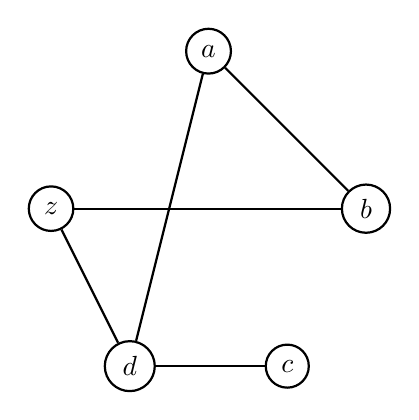
\begin{tikzpicture}[]
    \begin{scope}[every node/.style={circle,thick,draw}]
      \node (a) at (2,4) {$a$};
      \node (b) at (4,2) {$b$};
      \node (c) at (3,0) {$c$};
      \node (d) at (1,0) {$d$};
      \node (z) at (0,2) {$z$};
    \end{scope}
    \begin{scope}[every edge/.style={draw=black,thick}]
      \path (a) edge (b);
      \path (a) edge (d);
      \path (b) edge (z);
      \path (c) edge (d);
      \path (d) edge (z);
    \end{scope}
  \end{tikzpicture}
  \end{figure}
  
  \begin{parts}
    \part Determine the vertex set.
    \part Determine the edge set.
    \part Determine the adjacency list.
    \part For each of the vertices, determine the degree.
  \end{parts}
  \begin{solution}
    \begin{parts}
    	\part $ \{ a, b, c, d, z \} $.
  		\part $ \{ \{a, b\}, \{a, d\}, \{b, z\}, \{c, d\} \{d, z\} \} $.
		  \part \begin{tabular}{r|lll} a & b & d & \\ b & a & z & \\ c & d & & \\ d & a & c & z \\ z & b & d & \end{tabular}
		  \part $a: 2, b: 2, c: 1, d: 3, z:2$.
  	\end{parts}
  \end{solution}

\question
	Professor McBrain and his wife April give a party at which there are four other married couples.
	Some pairs of people shake hands when they meet, but naturally no couple shake hands with each other.
	At the end of the party the Professor asks everyone else how many people they have shaken hands with, and he receives nine different answers.~\cite{biggs02}
	\begin{parts}
		\part Draw a graph representing the handshakes exchanged at the party.
		\part How many people shook hands with April?
	\end{parts}
	\begin{solution}
		\begin{center}
  	 \begin{adjustbox}{max width=0.6\textwidth}
	  	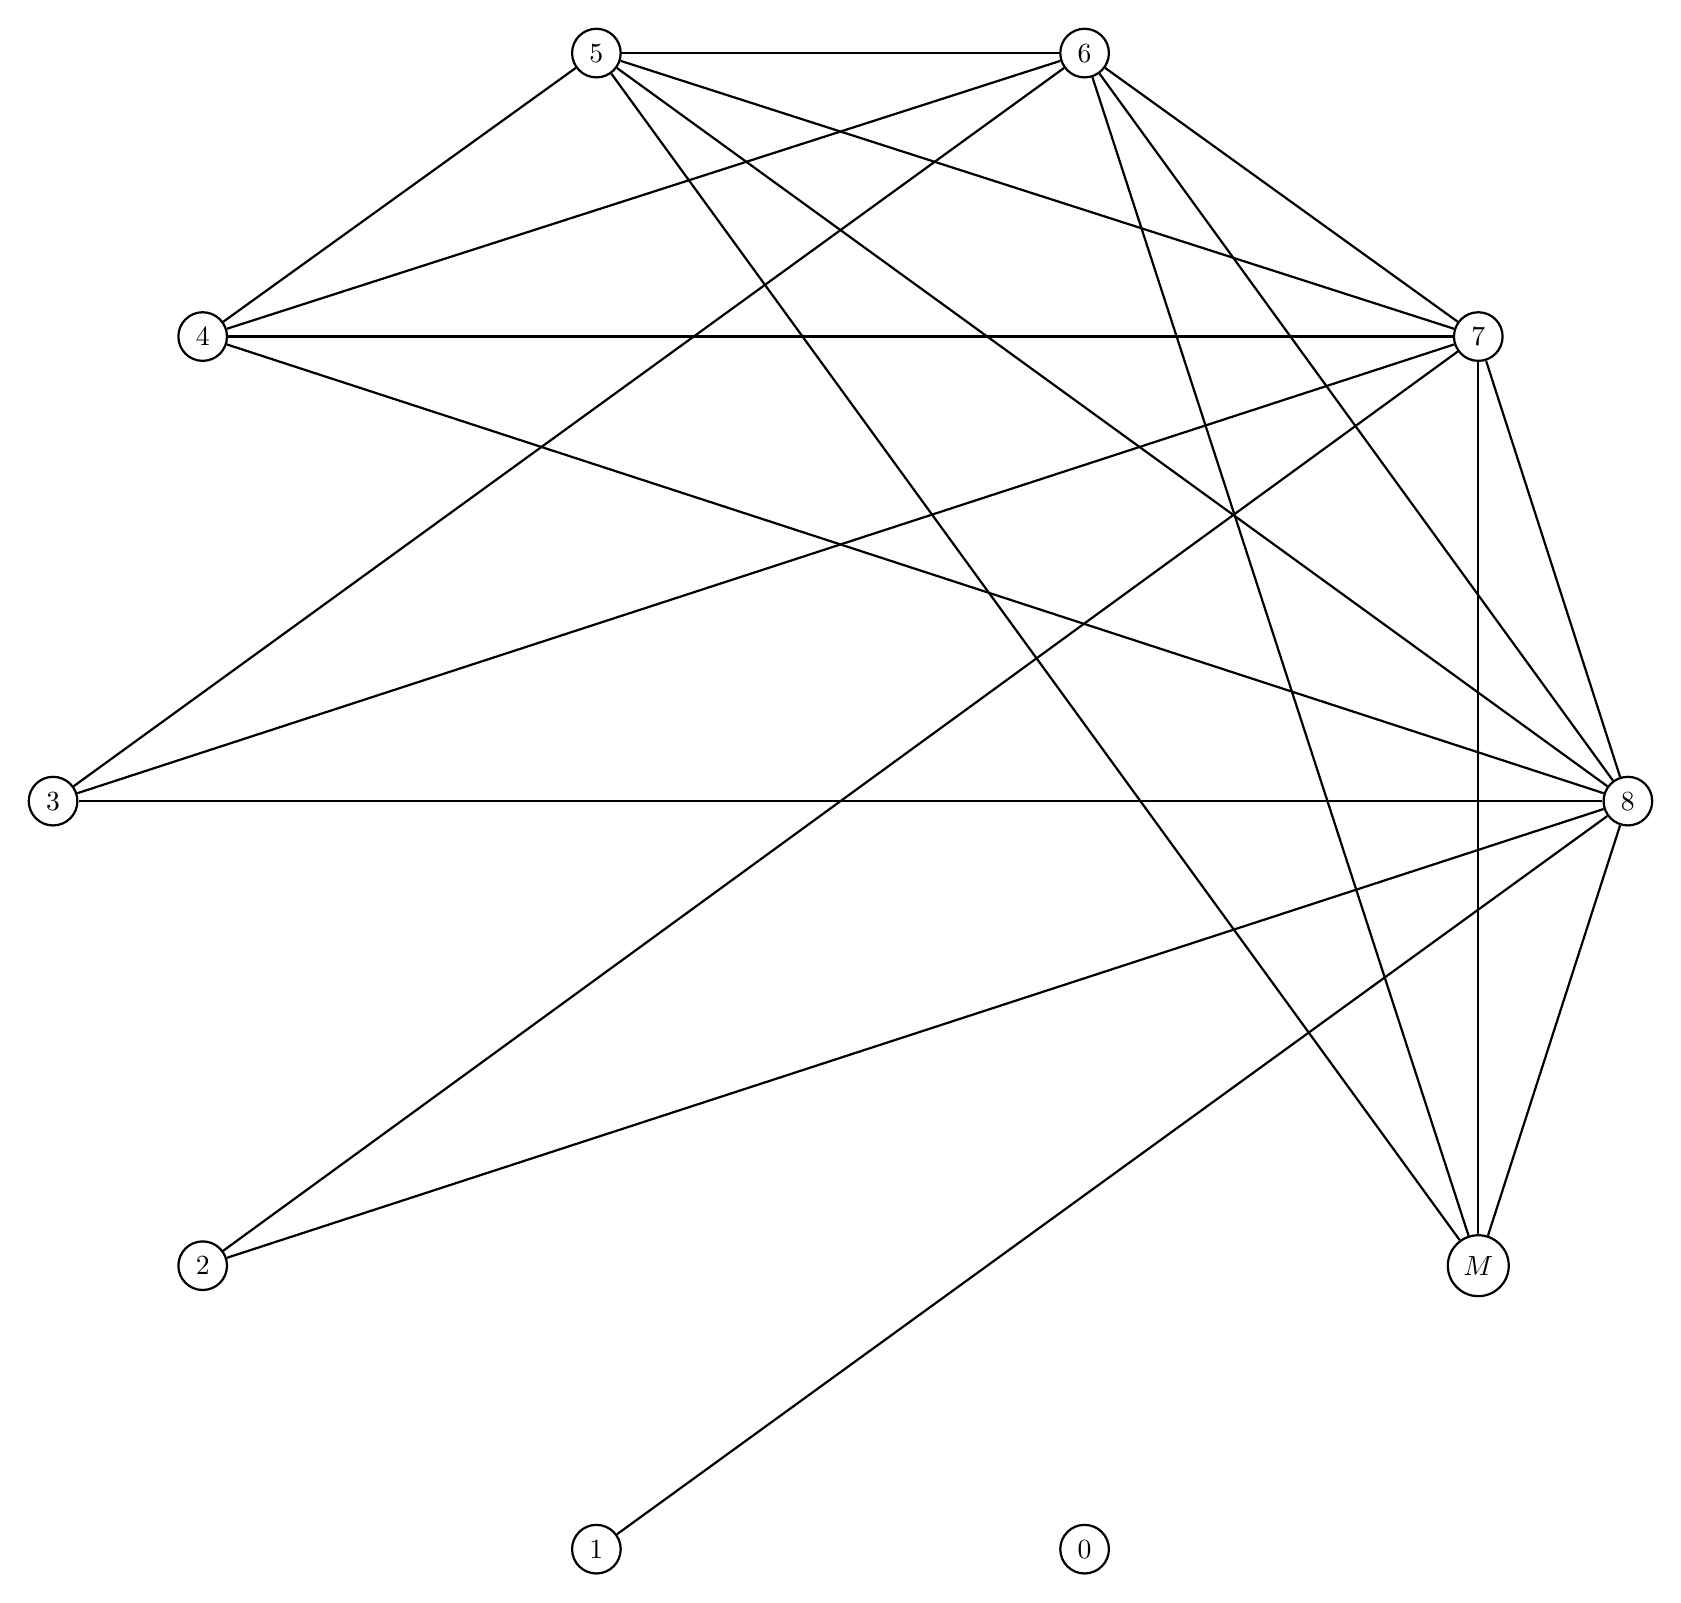
\begin{tikzpicture}
        \begin{scope}[every node/.style={circle,thick,draw}]
          \node (0) at (3.1,-9.5) {$0$};
          \node (1) at (-3.1,-9.5) {$1$};
          \node (2) at (-8.1,-5.9) {$2$};
          \node (3) at (-10.0,0) {$3$};
          \node (4) at (-8.1,5.9) {$4$};
          \node (5) at (-3.1,9.5) {$5$};
          \node (6) at (3.1,9.5) {$6$};
          \node (7) at (8.1,5.9) {$7$};
          \node (8) at (10.0,0) {$8$};
          \node (M) at (8.1,-5.9) {$M$};
          
        \end{scope}
        \begin{scope}[every edge/.style={draw=black,thick}]
          \path (8) edge (1);
          \path (8) edge (2);
          \path (8) edge (3);
          \path (8) edge (4);
          \path (8) edge (5);
          \path (8) edge (6);
          \path (8) edge (7);
          \path (8) edge (M);
          \path (7) edge (6);
          \path (7) edge (5);
          \path (7) edge (4);
          \path (7) edge (3);
          \path (7) edge (2);
          \path (7) edge (M);
          \path (6) edge (5);
          \path (6) edge (4);
          \path (6) edge (3);
          \path (6) edge (M);
          \path (5) edge (4);
          \path (5) edge (M);
        \end{scope}
  		\end{tikzpicture}
		\end{adjustbox}
		\end{center}

	
	We construct a graph whose vertices are the people at the party, and there is an edge (x, y) whenever x and y shook hands.
	Since there are nine people apart from Professor McBrain, and the maximum number of handshakes in which any one person can be involved is eight, it follows that the nine different answers received by the Professor must be 0, 1, 2, 3, 4, 5, 6, 7, 8.
	We denote the vertices by these numbers and use M for McBrain himself.
	So we have a pictorial representation.
	Now, vertex 8 is joined to all the other vertices except one, which must therefore represent the spouse of 8.
	This vertex must be 0, since it is certainly not joined to 8 (or any other vertex, for that matter).
	Thus 8 and 0 are a married couple, and 8 is joined to 1, 2, ..., 7 and M.
	In particular 1 is joined to 8 and this is the only edge from 1.
	Hence vertex 7 is not joined to 0 and 1 (only), and the spouse of 7 must be 1, since 0 is married to 8.
	Continuing in the same way, we see that 6 and 2, and 5 and 3 are married couples.
	It follows that M and 4 are married, so vertex 4 represents April, who shook hands with four people.
  \end{solution}

\question
Three houses A, B, C each has to be connected to the gas, water and electricity supplies: G, W, E.
Write own the adjacency list for the graph which represents this problem, and construct a pictorial representation of it.
Can you find a picture in which the lines representing the edges do not cross?~\cite{biggs02}

\question
The pathways in a formal garden are to be laid out in the form of a wheel graph $W_n$ whose vertex set is $V = \{0,1,2,\ldots,n\}$ and whose edges are:
\begin{align*}
	&\{0,1\}, \{0,2\}, \ldots, \{0,n\}, \\
	&\{1,2\}, \{2,3\}, \ldots, \{n-1,n\}, \{n,1\}
\end{align*}
Describe a route around the pathways which starts and ends at vertex 0 and visits every vertex once only.~\cite{biggs02}

\question
For each positive integer $n$ we define the complete graph $K_n$ to be the graph with n vertices in which each pair of vertices is adjacent.~\cite{biggs02}
\begin{parts}
	\part How many edges has $K_n$?
	\part For which values of $n$ can you find a pictorial representation of $K_n$ with the property that the lines representing the edges do not cross?
\end{parts}

\question
A 3-cycle in a graph is a set of three mutually adjacent vertices.
Construct a graph with five vertices and six edges which contains no 3-cycles.~\cite{biggs02}

\end{questions}

\begin{thebibliography}{9}

\bibitem{biggs02}
  Norman Biggs,
  \emph{Discrete Mathematics},
  Oxford University Press,
  2nd edition,
  2002.

\end{thebibliography}
